\documentclass{article}

\usepackage{graphicx}

\begin{document}

\title{Report: Shape Detection}
\maketitle

\seciton{Subtask 1: The No-Entry Sign Detector}
\subsection{Training performance}

\begin{figure}[!htb]
    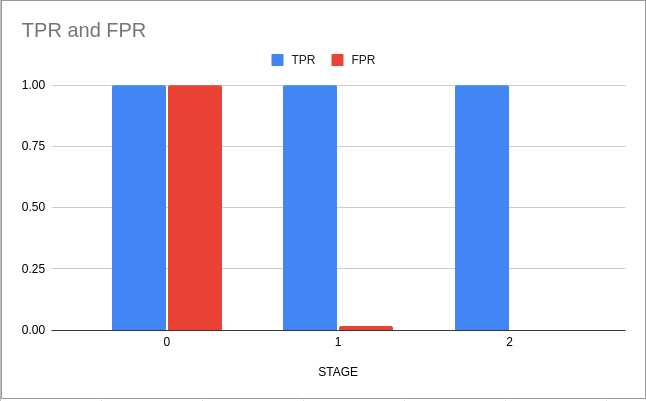
\includegraphics[width=\linewidth]{subtask1/trainingTPR_FPR.png}
    \caption{traning data}
    \label{fig:training}
\end{figure}

The Viola jones detection algorithm works by adding additional weak classifiers on each stage so naturally it starts accepting all images which gives it a 100\% acceptance rate for all images giving 1 for both TPR and FPR.
The next stages work by adding weak classifiers and they stopping accepting so many false positives.
The true positive rate achieved during testing is worse than that ahieved 

\subsection{Testing performance}

\begin{figure}
    \centering
    
    \subfigure(a){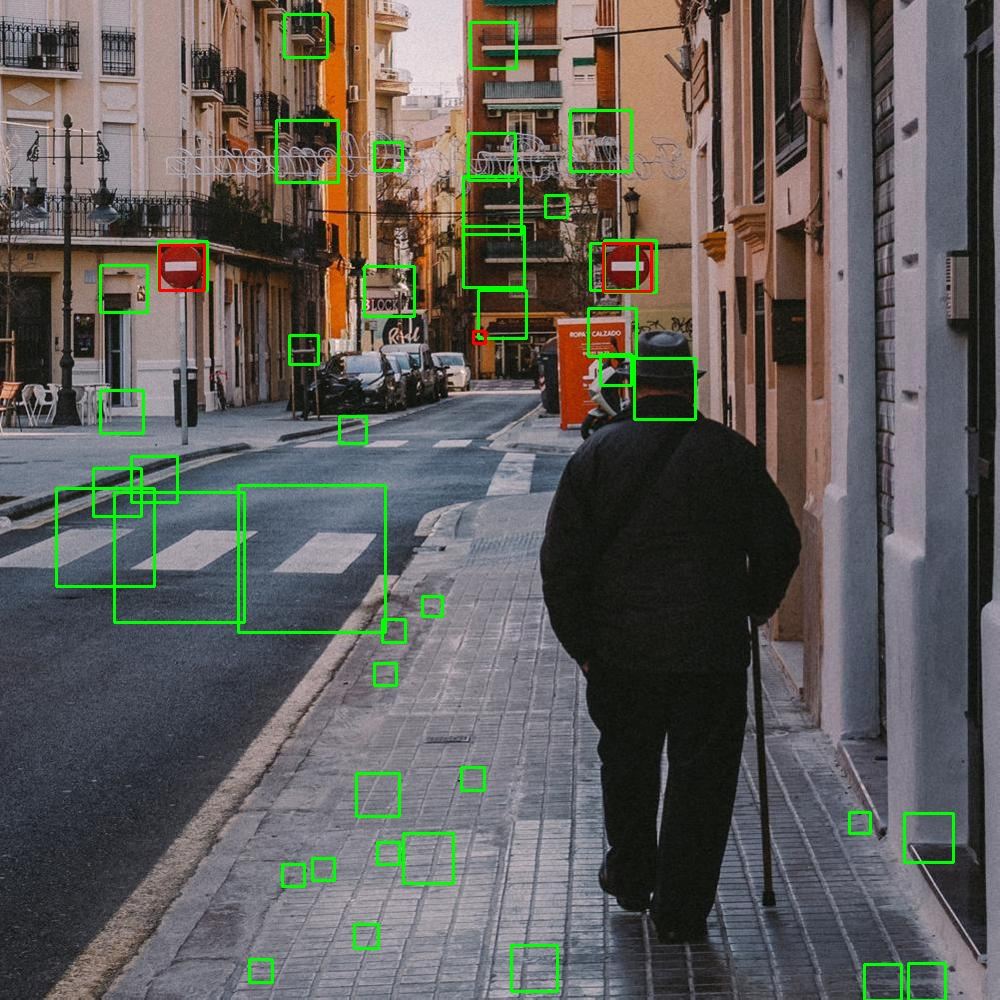
\includegraphics[width=50mm]{subtask1/result0.jpg}} 
    \subfigure(b){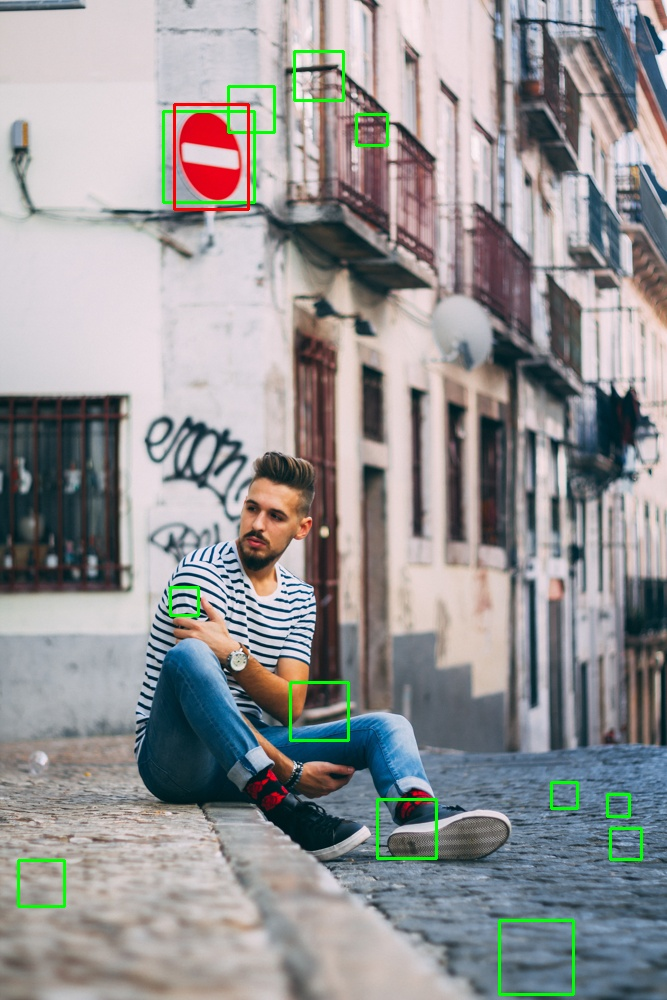
\includegraphics[width=50mm]{subtask1/result1.jpg}} 
    \subfigure(c){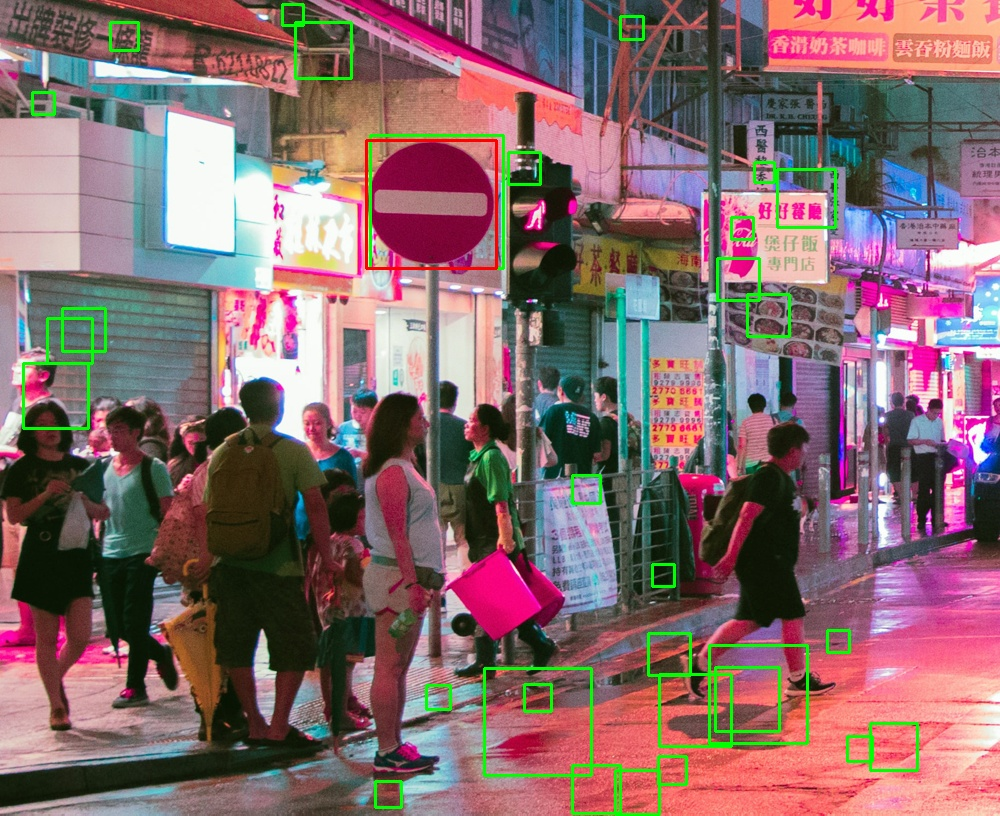
\includegraphics[width=50mm]{subtask1/result2.jpg}}
     
    \label{fig:foobar}
\end{figure}

\section{Subtask 2: Integration with Shape Detectors}



\end{document}